\documentclass[12pt,a4paper]{article}
\usepackage{inverba}

\newcommand{\userName}{Cullyn Newman} 
\newcommand{\class}{CH 334} 
\newcommand{\institution}{Portland State University} 
\newcommand{\theTitle}{\color{B-Cold} Apres Lecture Quizzes}
\begin{document}
%%%%%%%%%%%%%%%%%%%%%%%%%%%%%%%%%%%%%%%%%%%%%%%%%%%%%%%%%%%%%%%%%%%%%
\tableofcontents
\cleardoublepage
\fancyhead{}
%%%%%%%%%%%%%%%%%%%%%%%%%%%%%%%%%%%%%%%%%%%%%%%%%%%%%%%%%%%%%%%%%%%%%

%%%%%%%%%%%%%%%%%%%%%%%%%%%%% Week 7 %%%%%%%%%%%%%%%%%%%%%%%%%%%%%
%\begingroup
\section*{Week 7}\phantomsection
\addcontentsline{toc}{section}{\textbf{Week 7}}
\fancyhead[R]{\hyperlink{home}{Week 7}}

\fancyhead[L]{\hyperlink{home}{Tuesday, November 10 - Quiz 17}}
\subsection{Tuesday, November 10 - Quiz 17}
\begin{enumerate}
    {\color{G-Moon}\item Based on the Cahn Ingold Prelog rules, rank the following in order of lowest to highest priority.
    
    \ch{CH3}
    \hspace*{20pt}
    \ch{CH2CH3}
    \hspace*{20pt}
    \ch{CH2CH2OH}
    \hspace*{20pt}
    \ch{CH2CH2NH2}
    \hspace*{20pt}
    \ch{CH3CHO}
    }
        \begin{itemize}
            \item {\color{o-Sun}\textbf{\ch{CH3} < \ch{CH2CH3} < \ch{CH2CH2NH} < \ch{CH2CH2OH} < \ch{CH3CHO}}}
            \begin{itemize}
                \item Relevant notes (highlighted applies to this problem):
                    \begin{itemize}
                        \item \textbf{Chan-Ingold-Prelog system}: a system of nomenclature for Identifying each enantiomer individually.
                        \begin{enumerate}
                            {\color{o-Sun}\item Assign priorties to each of the four groups based on atomic number; the highest atomic number has the highest priority.}
                            \item Rotate the molecule so that the fourth priority group is on a dash (behind)
                            \item Determin the configuration, i.e., sequence of 1-2-3 groups.
                                \begin{itemize}
                                    \item {\color{true}clockwise (R)} or {\color{false}counterclockwise (S)}.
                                \end{itemize}
                        \end{enumerate}
                    {\color{o-Sun}\item If there is a tie between the atoms connected, then continue outward until a difference is found.}
                        \begin{itemize}
                            \item Do not add the sum all atomic numbers attached to each atom, just the first in which the atoms differ.
                           {\color{o-Sun}\item Any multiple bonded atom, (2 or 3) is treated as if connected to multiple atoms equal to number of bonds.}
                        \end{itemize} 
                    \end{itemize}
                \item First difference is the \ch{NH2} vs \ch{OH2}; oxygen has more mass.
                \item Leaves difference between \ch{CH2OH} vs \ch{CHO}; oxygen is double bonded in the latter, so really {CHOO} (O beats H).
            \end{itemize}
        \end{itemize}
    {\color{G-Moon}\item Determine the absolute configuration of the following molecule.
    
    \chemfig{\ch{H3C}-[:30](-[:91]\ch{OH})(<[:-60]\ch{CH2CH3})(<:[:-10]H)}
    
    }
        \begin{itemize}
            \item {\color{o-Sun}\textbf{R}}
            \begin{itemize}
                \item {\color{true}\chemfig{\ch{3}-[:30](-[:91]\ch{1})(<[:-60]\ch{2})(<:[:-10]4)}\hspace*{20pt} clockwise(R)}
                \item H = 4, \ch{CH3} = 3, \ch{CH2CH3} = 2, \ch{OH} = 1.
                \item Lowest priority is already in the back, leave as is.
            \end{itemize}
        \end{itemize}
    {\color{G-Moon}\item The molecule shown below is the enantiomer of the molecule shown in the previous question.  What is its absolute configuration?
    
    \chemfig{\ch{H3C}-[:30](-[:91]\ch{CH2CH3})(<[:-60]\ch{OH})(<:[:-10]H)}
    }
        \begin{itemize}
            \item {\color{o-Sun}\textbf{S}}
            \begin{itemize}
                \item \schemestart
                {\color{true}\chemfig{
                    \ch{3}-[:30](-[:91]\ch{1})(<[:-60]\ch{2})(<:[:-10]4)
                    }}
                \arrow{->}
                {\color{false}\chemfig{
                    \ch{3}-[:30](-[:91]\ch{2})(<[:-60]\ch{1})(<:[:-10]4)
                    }}
                \schemestop
                \item Swap 1 and 2, swap the configuration; \ch{R -> S}
            \end{itemize}
        \end{itemize}
    {\color{G-Moon}\item What is the absolute configuration of the molecule shown below?
    
    \chemfig{
        \ch{Br}-[:30](-[:91]\ch{CH3})(<[:-60]\ch{OH})(<:[:-10]\ch{CHO})
    }
    }
        \begin{itemize}
            \item {\color{o-Sun}\textbf{R}}
            \begin{itemize}
                \item \schemestart
                \chemfig{
                    \ch{1}-[:30](-[:91]\ch{4})(<[:-60]\ch{3})(<:[:-10]\ch{2})
                    }
                \arrow{->}
                {\color{true}\chemfig{
                    \ch{1}-[:30](-[:91]\ch{2})(<[:-60]\ch{3})(<:[:-10]\ch{4})
                    }}
                \schemestop
                \item Once lowest priority is assigned to dashed wedge(aka cram), then one can tell sequence. Original is an S.
            \end{itemize}
        \end{itemize}
\end{enumerate}

\newpage
\fancyhead[L]{\hyperlink{home}{Monday, November 9 - Quiz 16}}
\subsection{Monday, November 9 - Quiz 16}
\begin{enumerate}
    {\color{G-Moon}\item Which of the following molecules is not capable of existing in cis and trans isomeric forms?

    \chemfig{=[:30](-[:90])-[:-30]-[:30]}
    \hspace*{14pt}
    \chemfig{-[:30](-[:90])=[:-30]-[:30]}
    \hspace*{14pt}
    \chemfig{-[:30](-[:90])-[:-30]=[:30]}
    }
        \begin{itemize}
            \item {\color{o-Sun}\textbf{All of the above}} 
            \begin{itemize}
                \item Option 1 and 3 both have a $\pi$ bonded carbon (sp\(^{2}\)), which has two hydrogens as the substituents---compounds with same substituents on both sides are unable to be cis--trans.
                \item Likewise, option 2, has \ch{CH3} on both sides of one end of the $\pi$ bond, making them the have same substituents. 
            \end{itemize}
        \end{itemize}
    {\color{G-Moon}\item Which of the following molecules corresponds to a cis isomer?
    
    \chemfig{\ch{Cl}-[:90]-[:30](-[:90])-[:-30](-[-90]\ch{Cl})=[:30]}
    \hspace*{10pt}
    \chemfig{-[:30](-[:90])(-[:-90]\ch{Cl})-[:-30](-[-90]\ch{Cl})=[:30]}
    \hspace*{10pt}
    \chemfig{-[:30](-[:90]-[:30]\ch{Cl})(-[:-90]\ch{Cl})-[:-30]=[:30]}
    \hspace*{10pt}
    \chemfig{-[:30](-[:90])-[:-30](-[:-90]\ch{Cl})=[:30]-[:-30]}
    }
        \begin{itemize}
            \item {\color{o-Sun}\textbf{D}} 
            \begin{itemize}
                \item A, B, and C all cannot be cis--trans isomers due to double hydrogen substituents.
            \end{itemize}
        \end{itemize}
    {\color{G-Moon}\item What condition causes a carbon center to be classified as asymmetric?}
        \begin{itemize}
            \item {\color{o-Sun}\textbf{The C must have four different groups bonded to it}} 
            \begin{itemize}
                \item Asymmetric carbon center = \textbf{chiral center}, i.e., a tetrahedral carbon that bears four different groups.
            \end{itemize}
        \end{itemize}
    {\color{G-Moon}\item Suppose a sample of 2-methyl-1-butanol (see lecture notes), when placed in plane polarize light, showed a rotation of \ang{-4.32}. What is the enantiomeric excess of the enantiomer that rotates light to the left?}
        \begin{itemize}
            \item {\color{o-Sun}\textbf{75.1\%}} 
            \begin{itemize}
                \item \(\%~ee = \dfrac{|\text{observed}~(\alpha)|}{|\text{specific}~[\alpha]|} \times 100\%\)
                \item (from slides) 2-methyl-1-butanol: specific $[\alpha]^{\SI{20}{\celsius}}_D = \pm5.75$; observed \((\alpha) = -4.32\).  
                \item \(ee = \dfrac{\ang{4.32}}{\ang{5.75}} \times 100\% = 75.1\%\)
            \end{itemize}
        \end{itemize}
    {\color{G-Moon}\item While nature, i.e., enzymes, synthesize molecules with chiral centers in 100\% enantiomeric purity, that often proves very difficult for synthetic organic chemists to do.  What most often results in the lab is a mixture containing equal concentrations of both enantiomers. What term is used to describe this mixture?}
        \begin{itemize}
            \item {\color{o-Sun}\textbf{Racemic mixture}} 
            \begin{itemize}
                \item (from notes) \textbf{Racemic mixtrue}: a solution containing equal amounts of both enantiomers, resulting in an optically inactive appearance.
            \end{itemize}
        \end{itemize}
    {\color{G-Moon}\item What physical properties distinguish the R enantiomer from the S enantiomer of a molecule?}
        \begin{itemize}
            \item {\color{o-Sun}\textbf{they rotate plane polarized light in equal, but opposite, directions}} 
            \item Relevant notes:
                \begin{itemize}
                    \item Specific rotation for enantiomers are {\color{o-Sun}equal in magnitude} but {\color{o-Sun}opposite in direction}.
                        \begin{itemize}
                            \item {\color{pos}\textbf{dextrorotaory}}: a compound exhibiting {\color{pos}positive} rotation.
                            \item {\color{neg}\textbf{levorotatory}}: a compound exhibiting {\color{neg}negative} rotation.
                            \item No direct relationship between R/S system of nomenclature, as that is independent of conditions, but dependent on observation angle.
                            \item The {\color{o-Sun}direction} of polarized light, however, is {\color{o-Sun}dependent on conditions}, and can change based on temperature or wavelength even with the same given configuration.
                        \end{itemize}
                \end{itemize}
        \end{itemize}
\end{enumerate}

%\endgroup
%%%%%%%%%%%%%%%%%%%%%%%%%%%%% Week 7 %%%%%%%%%%%%%%%%%%%%%%%%%%%%%

%%%%%%%%%%%%%%%%%%%%%%%%%%%%% Week 6 %%%%%%%%%%%%%%%%%%%%%%%%%%%%%
%\begingroup
\clearpage
\section*{Week 6}\phantomsection
\addcontentsline{toc}{section}{\textbf{Week 6}}
\fancyhead[R]{\hyperlink{home}{Week 6}}

\fancyhead[L]{\hyperlink{home}{Monday, November 2}}
\subsection{Monday, November 2}
\begin{enumerate}
    {\color{G-Moon}\item What is the name of the following molecule?
    
    \chemfig{*6((-\ch{Br})---(-\ch{CH3})-(-\ch{Cl})--)}
    \vspace*{10pt}
    }
        \begin{itemize}
            \item {\color{o-Sun}\textbf{4-bromo-1-chloro-2-metyhlcyclohexane}}
            \begin{itemize}
                \item Lowest sum and alphabetically ordered.
            \end{itemize}
        \end{itemize}
    {\color{G-Moon}\item What is the definition of a molecular conformation?}
        \begin{itemize}
            \item {\color{o-Sun}\textbf{A geometric arrangement in space of a molecule that has a low energy pathway to rearrangement}}
            \begin{itemize}
                \item \textbf{Conformations}: the variety of possible three-dimensional shapes of a molecule that are interchangeable by low energy pathways.
                    \begin{itemize}
                        \item Conformations vary in potential energy.
                        \item Changes due to rotation about $\sigma$ bonds.
                    \end{itemize}
            \end{itemize}
        \end{itemize}
    {\color{G-Moon}\item What is the following molecule?
    
    (The package that draws newman projections is not compatable with the font I use... working on a fix, but can't draw them at the moment)
    }
        \begin{itemize}
            \item {\color{o-Sun}\textbf{pentane}}
            \begin{itemize}
                \item Front portion has 3 carbons in the chain: \ch{CH3} (1), \ch{CH2} (2), and the \ang{4} carbon (3) in the center.
                \item The circle represents the $\sigma$ bond between the carbon behind it, so thats (4).
                \item The methyl (\ch{CH3}) on the back portion is (5).
            \end{itemize}
        \end{itemize}
        \newpage
    {\color{G-Moon}\item For the molecule in the previous question, which conformer is the gauche form of the molecule?}
        \begin{itemize}
            \item {\color{o-Sun}\textbf{choice 1}}
            \item Can't draw newman projections currently; it's broken... but here's this lame screenshot:
            
            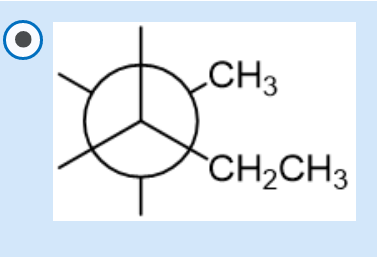
\includegraphics[scale=0.3]{images/newman1.png}
            \begin{itemize}
                \item \textbf{Gauche interaction}: unfavorable intereaction between groups, causing an increases in energy due to electron cloud repulsion.
                \item Gauche intereaction is a type of steric intereactions present at \(\approx\pm\ang{60}\) the next eclipsed conformation. 
                \end{itemize}
        \end{itemize}
    {\color{G-Moon}\item For the same molecule, which conformation corresponds to the most stable form?}
        \begin{itemize}
            \item {\color{o-Sun}\textbf{pick number 1 m'lord}}
            \item ugggghhhhhhhhhhhhhh so ugly :(
            
            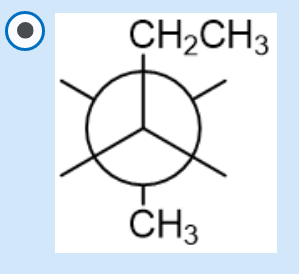
\includegraphics[scale=0.3]{images/newman2.png}
            \begin{itemize}
                \item Other forms represent an eclipsed form and the gauche interaction, both which increases potential energy due to increased torsional strain.
                \item More notes for reference:
                    \begin{itemize}
                        \item \textbf{dihedral (torsional) angle}: the angle between substituents of front and back carbons as the $\sigma$ bonds rotates.
                        \item \textbf{Staggered conformation}: {\color{o-Sun}lowest energy} conformation, when two substituents are at maximum dihedral angle from each other.
                        \item \textbf{Eclipsed conformation}: the {\color{o-Sun}highest energy} conformation, when two substituents are at the minimum dihedral angle from each other.
                    \end{itemize}
            \end{itemize}
        \end{itemize}
    \newpage
    {\color{G-Moon}\item For which molecule will the energy of conversion (E\(_{\text{act}}\)) be the greatest?}
        \begin{itemize}
            \item {\color{o-Sun}\textbf{butane}}
            \begin{itemize}
                \item I don't really know what E\(_{\text{act}}\) is, but I assume it's the energy required to go through the interchangeable pathway.
                \item Costs of butane: 
                    \begin{itemize}
                        \item \SI{19}{kJ\per\mole} (eclipsed with methyl overlap; once) 
                        \item \SI{16}{kJ\per\mole} (eclipsed, no methyl, but with gauche; twice)
                        \item \SI{3.8}{kJ\per\mole} (gauche only; twice)
                    \end{itemize}
                \item I'm not sure if you add them up or just take max, but either way butane has the greatest out of ethane, propane, and methane.
            \end{itemize}
        \end{itemize}
    {\color{G-Moon}\item Why is the cyclohexane ring more stable than rings of other sizes?
    \begin{itemize}
        \item the bond angles are all nearly \ang{109.5}
        \item the ring strain is at a minimum
        \item the overlap of the sp\(^{3}\) hybrid orbitals is at a maximum
    \end{itemize}}
        \begin{itemize}
            \item {\color{o-Sun}\textbf{all of the above}}
            \begin{itemize}
                \item This is true in the most stable, chair conformaions at least.
            \end{itemize}
        \end{itemize}
    {\color{G-Moon}\item Why can't the cyclobutane ring be square planar?}
        \begin{itemize}
            \item {\color{o-Sun}\textbf{the sp\(^{3}\) orbitals wouldn't overlap well}}
            \begin{itemize}
                \item Cyclobutane adopts a slightly puckered conformation in order to reduce angle strain (and eclipsed H)... which I guess are the sp\(^{3}\) orbitals. I got this wrong multipile times; need to review orbitals I guess.
            \end{itemize}
        \end{itemize}
    {\color{G-Moon}\item In the cartoon picture shown below, who's on the chair and who's on the boat forms of cyclohexane?}
        \begin{itemize}
            \item {\color{o-Sun}\textbf{she's on the chair and he's on the boat}}
            \begin{itemize}
                \item Hmmmmmmmmmmmm....
            \end{itemize}
        \end{itemize}
    {\color{G-Moon}\item What is the total energy for the cyclohexane ring flipping process?}
        \begin{itemize}
            \item {\color{o-Sun}\textbf{12.1}}
            \begin{itemize}
                \item Appears to be just the cost of the first flip to the half chair.
                \item Can't seem to find good explanation to why, however.
            \end{itemize}
        \end{itemize}
\end{enumerate}
%\endgroup
%%%%%%%%%%%%%%%%%%%%%%%%%%%%% Week 6 %%%%%%%%%%%%%%%%%%%%%%%%%%%%%

%%%%%%%%%%%%%%%%%%%%%%%%%%%%% Week 5 %%%%%%%%%%%%%%%%%%%%%%%%%%%%%
%\begingroup
\clearpage
\section*{Week 5}\phantomsection
\addcontentsline{toc}{section}{\textbf{Week 5}}
\fancyhead[R]{\hyperlink{home}{Week 5}}

\fancyhead[L]{\hyperlink{home}{Friday, October 30}}
\subsection{Friday, October 30}
\begin{enumerate}
    {\color{G-Moon}\item The name of the molecule shown below is
    
    \chemfig{-[:30](\chembelow[1ex]{}{2}-[:90])-[:-30]-[:30](\chembelow[1ex]{}{4}-[:90])-[:-30]-[:30]-[:-30]\chembelow[1ex]{}{7}}
    }
        \begin{itemize}
            \item {\color{o-Sun}\textbf{2,4-dimethylheptane}}
                \begin{itemize}
                    \item Parnet chain, 7---heptane.
                    \item Two methyl groups---dimethyl 
                    \item Locations of methyls---2,4
                \end{itemize}
        \end{itemize}
    {\color{G-Moon}\item What is incorrect about the name, 3-butylpentane, for the following molecule?
    
    \chemfig{-[:30,,,,,line width=1pt]-[:-30,,,,,line width=1pt](-[:30]-[:-30])-[:-90,,,,,line width=1pt]-[:-30,,,,,line width=1pt]-[:30,,,,,line width=1pt]-[:-30,,,,,line width=1pt]}
    }
        \begin{itemize}
            \item {\color{o-Sun}\textbf{the longest chain is a heptane}}
        \end{itemize}
    {\color{G-Moon}\item What is the name of the following molecule?
    
    \chemfig{*6(-(-[:-90])--(-[:30]-[:-30])---)}
    }
        \begin{itemize}
            \item {\color{o-Sun}\textbf{1-ethyl-3-methylcyclohexane}}
                \begin{itemize}
                    \item Parnet chain: cyclohexane
                    \item One ethyl, one methyl.
                    \item First substituent receives lowest number, but if there is a tie then number is assigned alphabetically; starts with 1-ethyl.
                \end{itemize}
        \end{itemize}
    {\color{G-Moon}\item What is the name of the following molecule?
    
    \chemfig{*6(-(-[:-90])--(-[:30](-[:90])-[:-30])---)}
    }
        \begin{itemize}
            \item {\color{o-Sun}\textbf{1-isopropyl-3-methylcyclohexane}}
                \begin{itemize}
                    \item Parent chain: cyclohexane
                    \item One isopropyl (name for complex substituent bearing three carbons, aka 1-methylpropyl), one methyl.
                    \item Same as before, i is before m.
                \end{itemize}
        \end{itemize}
    {\color{G-Moon}\item What is the name of the following molecule?
    
    \chemfig{-[:-30]-[:30]-[:-30]-[:30]-[:-30](-[:30]-[:-30]-[:30]-[:-30])-[:-90](-[:210])-[:-30]-[:30]}
    }
        \begin{itemize}
            \item {\color{o-Sun}\textbf{5-sec-butyldecane}}
                \begin{itemize}
                    \item Parent chain: decane
                    \item one sec-butyl (1-methylpropyl)
                    \item Lowest locant(location of a carbon on a numbered parent chain): 5
                \end{itemize}
        \end{itemize}
    {\color{G-Moon}\item What is the name of the following molecule?
    
    \chemfig{-[:30]-[:-30](-[:-90,,,,,line width=1pt]-[:210,,,,,line width=1pt]-[:-90,,,,,line width=1pt])-[:30,,,,,line width=1pt](-[:90](-[::60])-[::-60])-[:-30,,,,,line width=1pt](-[:30,,,,,line width=1pt]-[:-30,,,,,line width=1pt]-[:30,,,,,line width=1pt]-[:-30,,,,,line width=1pt])-[:-90](-[:210])-[:-30]}
    }
        \begin{itemize}
            \item {\color{o-Sun}\textbf{4-ethyl-5,6-diisopropyldecane}}
                \begin{itemize}
                    \item Parent chain: decane
                    \item 1 ethyl, 2 isopropyl (1-methylpropyl)
                    \item Alphabetical tiebreaker again, 4-ethyl wins. 
                \end{itemize}
        \end{itemize}
    {\color{G-Moon}\item For any two molecules to be constitutional isomers of each other, they must have}
        \begin{itemize}
            \item {\color{o-Sun}\textbf{the same molecular formula}}
                \begin{itemize}
                    \item Constitutional isomers have the same molecular formula, different systematic names, and different atom connectivity.
                \end{itemize}
        \end{itemize}
    {\color{G-Moon}\item Why aren't hexane and cyclohexane constitutional isomers?}
        \begin{itemize}
            \item {\color{o-Sun}\textbf{all of the above}}
                \begin{itemize}
                    \item cyclohexane is missing 2 H due to \ch{C-C} bond making it a ring, which the chemical formula different and HDI different... also different names.
                \end{itemize}
        \end{itemize}
    {\color{G-Moon}\item Which molecule(s) represents a constitutional isomer of propylcyclohexane?}
        \begin{itemize}
            \item {\color{o-Sun}\textbf{all of the above}}
                \begin{itemize}
                    \item Propylcyclohexane: \hspace*{12pt} \chemfig{*6(---(-[::-60]-[::-60]-[::60])---)}
                    \item \chemfig{*6(---(-[:30](-[::60])-[::-60])---)}
                    \hspace*{12pt}
                    \chemfig{*6(--(-[::-60])-(-[::-60])-(-[::-60])--)}
                    \hspace*{12pt}
                    \chemfig{*6(--(-[::-60]-[::60])-(-[::-60])---)}
                \end{itemize}
        \end{itemize}
    {\color{G-Moon}\item 2,2-dimethylpropane and pentane represent}
        \begin{itemize}
            \item {\color{o-Sun}\textbf{constitutional isomers}}
                \begin{itemize}
                    \item \ch{C5H12}, pentane, can be arranged in three ways.
                    \item \chemfig{-[:-30]-[:30]-[:-30]-[:30]}
                    ~~
                    \chemfig{-[:-30](-[:-90])-[:30]-[:-30]}
                    ~~
                    \chemfig{-[:-30](-[:-120])(-[:-45])-[:30]}
                \end{itemize}
        \end{itemize}
\end{enumerate}

\newpage
\fancyhead[L]{\hyperlink{home}{Wednesday, October 28}}
\subsection{Wednesday, October 28}
\begin{enumerate}
    {\color{G-Moon}\item Comparing the following, which is the strongest acid?}
        \begin{itemize}
            \item {\color{o-Sun}\textbf{\ch{CH3COOH} \(pK_a\) = 4.8}}
                \begin{itemize}
                    \item \(pK_a\) generally ranges from {\color{pos}-10 (strong acid: positive charge)} to {\color{neg}50 (strong base: negative charge)}.
                \end{itemize}
        \end{itemize}
    {\color{G-Moon}\item Which of the following alcohols would you predict to be the most acidic?}
        \begin{itemize}
            \item {\color{o-Sun}\textbf{\ch{FH2COH}}}
                \begin{itemize}
                    \item Flourine has the greatest electronegativity compared to bromine and chlorine.
                    \item Inductive effect of the electronegative atom withdrawls more of the negative charge, making the conjugate base more stable (weaker).
                    \item Weaker conjugate base = stronger acid.
                \end{itemize}
        \end{itemize}
    {\color{G-Moon}\item Why is \ch{H-C+C-H} (\(pK_a\) = 25) more acidic than \ch{H2C=CH2} (\(pK_a\) = 44)?}
        \begin{itemize}
            \item {\color{o-Sun}\textbf{the \ch{H-C+C-} anion is more stable than \ch{H2C=CH-}}}
                \begin{itemize}
                    \item sp-hybridization of carbon results in a triple bond, while sp\(^{2}\) results in a double bond.
                    \item The negative charge on carbon anion is more stable when closer the the positive nucleus in a triple bond vs a double bond.
                    \item More stable (weaker) conjugate base (deprotonated molecule) results in stronger acid. 
                \end{itemize}
        \end{itemize}
    {\color{G-Moon}\item Why is \ch{CH3CH2CH2CHBrCOOH} (\(pK_a\) = 2.97) nearly two orders of magnitude less acidic than \ch{CH2BrCH2CH2CH2COOH} (\(pK_a\) = 4.71),  }
        \begin{itemize}
            \item {\color{o-Sun}\textbf{the inductive effect of Br is more pronounced in \ch{CH3CH2CH2CHBRCOOH} than in \ch{CH2BRCH2CH2CHCOOH}}}
                \begin{itemize}
                    \item The further the electronegative atom (\ch{Br}) causing the inductive effect from the deprotonated atom (\ch{O}), the less stable (stronger) conjugate base and the weaker the acid. 
                \end{itemize}
        \end{itemize}
    {\color{G-Moon}\item The greater acidity of a carbolic acid, \ch{RCOOH} (\(pK_a\) = 4.76) compared to an alcohol, \ch{ROH} (\(pK_a\) = 16) can almost entirely be attributed to}
        \begin{itemize}
            \item {\color{o-Sun}\textbf{the resonance stabilization of the \ch{RCOO-} anion compared to the \ch{RO-} anion}}
                \begin{itemize}
                    \item The two oxygen atoms allows for electron delocalization, increasing stability of the conjugate base, resulting in a stronger acid.
                    \item No delocalization is possible in the \ch{RO-}; the negative charge is stuck only on the one oxygen.
                \end{itemize}
        \end{itemize}
    {\color{G-Moon}\item We are going to see that most reactions in organic chemistry do not involve the H+ ion (from a Br{\o}nsted acid), other than as a catalyst.  Instead, reactions are viewed in terms of the interaction between a Lewis acid and a Lewis base.  Which of the following statements is true?}
        \begin{itemize}
            \item {\color{o-Sun}\textbf{a Br{\o}nsted acid is also a Lewis acids}}
                \begin{itemize}
                    \item All Bro{\o}nsted acids are also lewis acids, but the reverse is not always true.
                    \item An \ch{H+} ion can be a lewis acid, as it can accept a pair of electrons.
                \end{itemize}
        \end{itemize}
    {\color{G-Moon}\item Which of the following shows the correct way to draw the curved arrows for the indicated reaction?}
        \begin{itemize}
            \item {\color{o-Sun}\textbf{\ch{CH3-} 
            \begin{tikzpicture}
                \draw (0,0) node (^-) {};  
                \draw (1,0) node (^+) {};  
                    \path[->, draw, thick] (^-) to [bend left=45] (^+);
            \end{tikzpicture}
            \ch{^+CH3 -> CH3CH3}}}
                \begin{itemize}
                    \item {\color{neg}Tail} of arrow goes on {\color{neg}negative charge}, indicating {\color{neg}electron donor (base)}.
                    \item {\color{pos}Head} of arrow goes on {\color{pos}positive charge}, indicating {\color{pos}electron acceptor (acid)}.  
                \end{itemize}
        \end{itemize}
\end{enumerate}
%\endgroup
%%%%%%%%%%%%%%%%%%%%%%%%%%%%% Week 5 %%%%%%%%%%%%%%%%%%%%%%%%%%%%%

%%%%%%%%%%%%%%%%%%%%%%%%%%%%% Week 4 %%%%%%%%%%%%%%%%%%%%%%%%%%%%%
%\begingroup
\clearpage
\section*{Week 4}\phantomsection
\addcontentsline{toc}{section}{\textbf{Week 4}}
\fancyhead[R]{\hyperlink{home}{Week 4}}

\fancyhead[L]{\hyperlink{home}{Friday, October 23}}
\subsection{Friday, October 23}
\begin{enumerate}
    {\color{G-Moon}\item \ch{H3PO4} can lose one, two, or three protons. When it loses just one proton, what is the conjugate base?}
        \begin{itemize}
            \item {\color{o-Sun}\textbf{\ch{H2PO4-}}}
                \begin{itemize}
                    \item Removing a {\color{pos}\ch{H^+}} reduces H by one and {\color{neg}decreases charge} on the now deprotonated molecule by one.
                \end{itemize}
        \end{itemize}
    {\color{G-Moon}\item Acetic acid, \ch{CH3COOH}, has a \(pK_a\) of 4.76 while phenol, C6H5OH, has a \(pK_a\) of 9.4.  Which is the strongest acid?}
        \begin{itemize}
            \item {\color{o-Sun}\textbf{acetic acid}}
                \begin{itemize}
                    \item \(pK_a\) generally ranges from {\color{pos}-10 (strong acid: positive charge)} to {\color{neg}50 (strong base: negative charge)}.
                \end{itemize}
        \end{itemize}
    {\color{G-Moon}\item In the following reaction, is \ch{H2O} acting as an acid, base, or neither?}
        \begin{itemize}
            \item {\color{o-Sun}\textbf{base}}
                \begin{itemize}
                    \item {\color{pos}acid} + {\color{neg}base} \ch{<>} {\color{neg}conjugate base} + {\color{pos}conjugate acid}
                    \item Symbolically: {\color{pos}HA} + {\color{neg}B} \ch{<>} {\color{neg}\ch{A^-}} + {\color{pos}\ch{HB^+}}
                    \item Our case: {\color{pos}\ch{CH3COOH}} + {\color{neg}\ch{H2O}} \ch{<>} {\color{neg}\ch{CH3COO-}} + {\color{pos}\ch{H3O+}}
                \end{itemize}
        \end{itemize}
    {\color{G-Moon}\item In the following reaction, is \ch{H2O} functioning as an acid, a base, or neither?}
        \begin{itemize}
            \item {\color{o-Sun}\textbf{acid}}
                \begin{itemize}
                    \item Our case: {\color{neg}\ch{CH3NH2}} + {\color{pos}\ch{H2O}} \ch{<>} {\color{pos}\ch{CH3NH3+}} + {\color{neg}\ch{OH-}}
                \end{itemize}
        \end{itemize}
    {\color{G-Moon}\item In a reaction of an acid with a base, equilibrium is favored if}
        \begin{itemize}
            \item {\color{o-Sun}\textbf{the reaction proceeds from a stronger acid to a weaker acid}}
                \begin{itemize}
                    \item Equilibrium {\color{o-Sun}favors formation} of the {\color{o-Sun} weaker} (higher \(pK_a\)) {\color{o-Sun}acid}.
                    \item Favored means to have the reaction proceed in a particular direction. Once it's reached nothing is favored. That means you need a stronger base $\rightarrow$ weaker acid to have a favored direction.
                \end{itemize}
        \end{itemize}
    \newpage
    {\color{G-Moon}\item Which of the following statements is true?}
        \begin{itemize}
            {\color{G-Moon}\item[A.] a strong acid will produce a strong conjugate base
            \item[B.] a weak acid will produce a weak conjugate base
            \item[C.] a weak acid will produce a strong conjugate base
            \item[D.] a strong acid will produce a weak conjugate base.}
            \item {\color{o-Sun}\textbf{both C and D are true}}
                \begin{itemize}
                    \item The strength of the acid/base is {\color{o-Sun}inversley proportional} to the strength of the conjugate acid/base.
                \end{itemize}
        \end{itemize}
    {\color{G-Moon}\item Based upon the information given in Table 1 (chapter 6) in Strongin's book, will equilibrium favor the reactants or the products in the following reaction?
    
    \ch{NH3 + H2O -> NH4+ + OH-}\\
    \hspace{1pt} 36 \hspace{66pt} 9.4
    }
        \begin{itemize}
            \item {\color{o-Sun}\textbf{reactants}}
                \begin{itemize}
                    \item \(pK_a\) for \ch{NH4+} is 9.4 and \(pK_a\) for \ch{NH3} is 36 --- Thanks @Winterho\_\_\_ for numbers, I have no access to the book.
                    \item Equilibrium {\color{o-Sun}favors formation} of the {\color{o-Sun} weaker} (higher \(pK_a\)) {\color{o-Sun}acid}.
                \end{itemize}
        \end{itemize}
\end{enumerate}


\newpage
\fancyhead[L]{\hyperlink{home}{Wednesday, October 21}}
\subsection{Wednesday, October 21}
\begin{enumerate}
    {\color{G-Moon}\item A common reaction for carbonyls occurs by removing an alpha hydrogen to generate a carbanion, as shown for 2,4-pentanedione.  Most \ch{C-H} bonds are not acidic enough to react with any base, no matter how strong the base.  Why do you think that this happens in 2,4-pentanedione?
    
    \schemestart
    \chemfig{-[:30](=[:90]O)-[:-30]\chembelow[1ex]{}{\alpha}-[:30](=[:90]O)-[:-30]}
    \arrow{->[srong base]}
    \chemfig{-[:30](=[:90]O)-[:-30]\chembelow[1ex]{}{\circleddash}-[:30](=[:90]O)-[:-30]}
    \schemestop}
    \vspace{10pt}
        \begin{itemize}
            \item {\color{o-Sun}\textbf{the negative charge is resonance stabilized over two \ch{C=O} bonds}}
                \begin{itemize}
                    \item The negative charge on the carbanion can be pushed to the double bond between the carbon and the oxygen, which then pushes those electrons into lone pairs around the oxygen.
                    \item {\color{neg}Negative charges} prefer to be on the {\color{neg}most electronegative} element, in this case oxygen.
                    \item Both \ch{C=O} bonds can share the charge, as sharing between each one forms separate resonance structures that form together form the resonance hybrid. 
                \end{itemize}
        \end{itemize}
    {\color{G-Moon}\item Most alcohols, \ch{ROH}, are not very acidic, an exception is phenol, \ch{ArOH}, which is "mildly" acidic.  Including the starting structure, how many resonance forms can be drawn for the benzylic anion (shown below)?
    
    \chemfig{*6(-=-(-[:30]O^\circleddash)=-=)}
    \vspace{6pt}
    }
    \begin{itemize}
        \item {\color{o-Sun}\textbf{5}}
    \end{itemize}
    \vspace{10pt}
        \schemestart
        \chemfig{*6(-=[,,,,b-Ocean]-(-[:30]O^\circleddash)=[,,,,g-Leaf]-=[,,,,v-Haze])}
        \arrow{<->}
        \chemfig{*6(=[,,,,v-Haze]-=[,,,,b-Ocean](-[:30]O^\circleddash)-=[,,,,g-Leaf]-)}
        \arrow{<->}
        \schemestop
        \\
        \schemestart
        \chemfig{*6(=[,,,,v-Haze]-\chembelow[1ex]{}{\ominus}-(=[:30]O)-=[,,,,g-Leaf]-)}
        \arrow{<->}
        \chemfig{*6(\chembelow[1ex]{}{\ominus}-=[,,,,g-Leaf]-(=[:30]O)-=[,,,,b-Ocean]-)}
        \arrow{<->}
        \chemfig{*6(-=[,,,,b-Ocean]-(=[:30]O)-\chemabove[1ex]{}{\ominus}-=[,,,,v-Haze])}
        \schemestop
    \newpage
    {\color{G-Moon}\item For the molecule in the previous question,  how will the \ch{C-O} bond length compare to \ch{C-O} single bonds and \ch{C=O} double bonds?}
        \begin{itemize}
            \item {\color{o-Sun}\textbf{shorter than a single bond and longer than a double bond}}
                \begin{itemize}
                    \item Electron delocalization around the ring makes the \ch{C-O} in the stronger than a normal single bond, but weaker than a double bond.
                    \item The stronger the bond, the shorter the length.
                    \item So after delocalization its now {\color{o-Sun}shorter/stronger} than \ch{C-O}, but {\color{o-Sun}longer/weaker} than \ch{C=O}.
                \end{itemize}
        \end{itemize}
    {\color{G-Moon}\item For the molecule 1-fluorobutane, on which carbon will the inductive effect of the F be most prominent?

    \vspace{24pt}
    \chemfig{\chembelow[1ex]{}{4}-[:30]\chemabove[1ex]{}{3}-[:-30]\chembelow[1ex]{}{2}-[:30]\chemabove[1ex]{}{1}-[:-30]F}
    \vspace{12pt}
    }
        \begin{itemize}
            \item {\color{o-Sun}\textbf{1}}
            \begin{itemize}
                \item Inductive effects only influence atoms they are bonded to due to unequal sharing of electrons.
            \end{itemize}
        \end{itemize}
\end{enumerate}

\newpage
\fancyhead[L]{\hyperlink{home}{Monday, October 19}}
\subsection{Monday, October 19}
\begin{enumerate}
    {\color{G-Moon}\item When electrons are delocalized over several carbon centers, this results in}
        \begin{itemize}
            \item {\color{o-Sun}\textbf{greater stability of the molecule}}
                \begin{itemize}
                    \item Resonance allows for delocalization of electrons, which spreads the charge between multiple atoms and lowers overall energy of molecule; termed {\color{o-Sun}resonance stabilization}.
                \end{itemize}
        \end{itemize}
    {\color{G-Moon}\item When showing electron movement with curved arrows,}
        \begin{itemize}
            \item {\color{o-Sun}\textbf{the arrow head points towards the lewis acid}}
                \begin{itemize}
                    \item the tail "pushes" {\color{neg}electrons} from a {\color{neg}electronegative (lewis base:donor)} towards the {\color{pos}less electronegative (lewis acid:acceptor)}. 
                \end{itemize}
        \end{itemize}
    {\color{G-Moon}\item For electron delocalization, which of the following is allowed?}
        \begin{itemize}
            {\color{G-Moon} \item electrons can move from a lone pair to an sp\(^{2}\) hybridized carbon.
            \item electrons can move as a pair form an anion to an sp\(^{2}\) hybridized carbon.
            \item electrons can move from pi bonding orbitals to an sp\(^{2}\) hybridized carbon.}
        \end{itemize}
        \begin{itemize}
            \item {\color{o-Sun}\textbf{all of the above}}
                \begin{itemize}
                    \item No good explanation. I don't think of it in terms of hybridized carbons. 
                \end{itemize}
        \end{itemize}
    {\color{G-Moon}\item What is wrong with the electron movement shown in the following} 
        \begin{itemize}
            \item {\color{o-Sun}\textbf{electrons cannot move towrds an sp\(^{3}\) hybridized carbon}}
                \begin{itemize}
                    \item electrons from $\pi$ bonding orbitals can move, just not towards a carbon with a full octet (sp\(^{3}\)).
                \end{itemize}
        \end{itemize}
    {\color{G-Moon}\item Is electron delocalization possible in the following molecule?
    
    \chemfig{=_[:30]-[:-30]-[:30]=_[:-30]}
    }
        \begin{itemize}
            \item {\color{o-Sun}\textbf{no}}
                \begin{itemize}
                    \item Currently the \ch{CH2} in the middle has a full octet. You can't move the electrons from the $\pi$ bonds
                    \item There would have to be a carbocation in order to move the electrons.
                \end{itemize}
        \end{itemize}
    \newpage
    {\color{G-Moon}\item Which of the following molecules will be resonance stabilized by electron delocalization?

    \hspace{15pt}
    \chemfig{*6(--=-=-)}
    \hspace{15pt}
    \chemfig{*6(-=--=-)}
    \hspace{15pt}
    \chemfig{*6(=---=-)}
    }
        \begin{itemize}
            \item {\color{o-Sun}\textbf{A and C}}
                \begin{itemize}
                    \item A and C can push the electrons twice, since they are conjugated bonds ($\pi$ bonds separated by a $\sigma$ bond).
                    \item B would be too, if there was a carbocation on either of the carbons with two $\sigma$ bonds.
                \end{itemize}
        \end{itemize}
    {\color{G-Moon}\item Acetamide exists in a delocalized form that results from the two resonance forms shown below.  Will the "real" structure be more like the one on the left, the one on the right, or an equal average of the two?

    \schemestart
    \chemfig{-[:30](=[:90]O)-[:-30]NH_2}
    \arrow{<->}
    \chemfig{-[:30](=[:90]O^\circleddash)-[:-30]NH_2^\oplus}
    \schemestop}
        \begin{itemize}
            \item {\color{o-Sun}\textbf{structure on the left}}
                \begin{itemize}
                    \item Rules for contributing significance, descending:
                    \begin{itemize}
                        \item The greatest number of filled octets.
                        \item The greatest number of covalent bonds.
                        \item {\color{o-Sun}Minimize formally charged atoms}.
                        \item Separation of unlike and like charges, minimized and maximized respectively.
                        \item Negative charges placed on the most electronegativity atoms, positive charges placed on the less electronegative atoms.
                        \item Do not deviate substantially from idealized bond lengths and angles.
                        \item Maintain aromatic substructures locally while avoiding anti-aromatic ones.
                    \end{itemize}
                \end{itemize}
        \end{itemize}
    {\color{G-Moon}\item Which statement(s) is(are) true?
    \begin{itemize}
        \item the more resonance structures, the greater the stability of the molecule.
        \item the more atoms over which the electrons can be delocalized, the greater the stability.
        \item when charges develop due delocalization, the structure with the negative charge on the most electronegative element is the most stable.
        \item a resonance structure in which all the atoms are neutral is more stable than one in which some of the atoms bear charges
    \end{itemize}}
    \begin{itemize}
        \item {\color{o-Sun}\textbf{all of the above}}
            \begin{itemize}
                \item see rules above on contributing significance; more of the major contributors result in more stability of the molecule, generally. 
            \end{itemize}
    \end{itemize}
\end{enumerate}
%\endgroup
%%%%%%%%%%%%%%%%%%%%%%%%%%%%% Week 4 %%%%%%%%%%%%%%%%%%%%%%%%%%%%%

%%%%%%%%%%%%%%%%%%%%%%%%%%%%% Week 3 %%%%%%%%%%%%%%%%%%%%%%%%%%%%%
%\begingroup
\clearpage
\section*{Week 3}\phantomsection
\addcontentsline{toc}{section}{\textbf{Week 3}}
\fancyhead[R]{\hyperlink{home}{Week 3}}

\fancyhead[L]{\hyperlink{home}{Friday, October 16}}
\subsection{Friday, October 16}
\begin{enumerate}
    {\color{G-Moon}\item What is the classification for the carbon centers, from left to right, in the following molecule?


    \hspace{15pt}\chemfig{\ang{1}-[:30]\ang{4}(-[:120])(-[:60])-[:-30]\ang{2}-[:30]\ang{3}(-[:90])-[:-30]-[:30]-[:-30]}
    }
    \begin{itemize}
        \item {\color{o-Sun}\textbf{\ang{1}, \ang{4}, \ang{2}, \ang{3}}}
    \end{itemize}
    {\color{G-Moon}\item What is the classification of the following alcohol?
    
    \hspace{15pt}\chemfig{-[:-30]-[:30]\ang{2}(-[:90]OH)-[:-30]}
    }
    \begin{itemize}
        \item {\color{o-Sun}\textbf{\ang{2}}}
            \begin{itemize}
                \item Two carbons are attached to the carbon with the alcohol.
            \end{itemize}
    \end{itemize}
    {\color{G-Moon}\item How is the following amine classified?


    \hspace{15pt}\chemfig{-[:30]-[:-30]NH-[:0]}
    }
    \begin{itemize}
        \item {\color{o-Sun}\textbf{\ang{2}}}
            \begin{itemize}
                \item \ch{CH3CH2NHCH3}, looks like a dimethylamine with an extra \ch{CH2}. I don't know nomenclature yet, but the functional group (\ch{NH}) remains the same. Has two carbons connected to it.
            \end{itemize}
    \end{itemize}
    {\color{G-Moon}\item Which of the following is NOT an intermolecular force (IMF)?}
        \begin{itemize}
            \item {\color{o-Sun}\textbf{covalent bonding}}
                \begin{itemize}
                    \item Any kind of bonding is not an intermolecular force. Hydrogen bonding isn't actually bonding, but instead just the strongest IMF mainly due to close proximity of charges compared to other IMFs.
                \end{itemize}
        \end{itemize}
    {\color{G-Moon}\item Which of the following is the strongest IMF?}
    \begin{itemize}
        \item {\color{o-Sun}\textbf{hydrogen bonding}}
            \begin{itemize}
                \item See above answer. 
            \end{itemize}
    \end{itemize}
    {\color{G-Moon}\item For a molecule to be polar, what conditions must exist?}
    \begin{itemize}
        \item {\color{o-Sun}\textbf{all of the above}}
            \begin{itemize}
                \item A molecule must a molecular dipole moment in order to be polar, which means two or more bonds must not cancel each other out. 
                \item Polar bonds must exist in order to create the net dipole moment.
                \item Has to have F O N Cl; I don't know why it must, but the other are true so this has to be true.
            \end{itemize}
    \end{itemize}
    {\color{G-Moon}\item Of the following molecules, which will have the largest LDFs?}
        \begin{itemize}
            \item {\color{o-Sun}\textbf{\chemfig{-[:30](-[:120])(-[:60])-[:-30]-[:30](-[:90])-[:-30]-[:30]-[:-30]}
            }}
                \begin{itemize}
                    \item London dispersion forces (LDF) related to moloar mass, so generally the larger and heavier the compound, then the more atoms there are to randomly create dipole moments.
                \end{itemize}
        \end{itemize}
    {\color{G-Moon}\item Which two molecules will be the least miscible?}
        \begin{itemize}
            \item {\color{o-Sun}\textbf{\ch{O2} and \ch{H2O}}}
                \begin{itemize}
                    \item Least miscible means least likely to form a homogeneous mixture.
                    \item "Like dissolves like" regarding to polar molecules, meaning polarity must match in order to become homogenous.
                    \item All other choices are either both polar or both nonpolar.
                \end{itemize}
        \end{itemize}
    {\color{G-Moon}\item Which molecule will have the highest boiling  point?
    
    \hspace{15pt}\chemfig{-[:30]-[:-30]NH-[:0]}
    \hspace{15pt}\chemfig{-[:30](=[:90]O)-[:-30]}
    \hspace{15pt}\chemfig{-[:-30]-[:30]-[:90]OH}
    }
    \begin{itemize}
        \item {\color{o-Sun}\textbf{C}}
            \begin{itemize}
                \item When comparing boling points of compounds, look for following factors:
                    \begin{itemize}
                        \item Any dipole-dipole interactions? (increases boiling point)
                        \item Formation of hydrogen bonds? (increase boling point)
                        \item Number of electrons. (more electrons, higher boiling point)
                        \item Number of carbon atoms. (more surface area, higher boiling point)
                        \item Degree of branching of compound. (more branching, more surface area)
                    \end{itemize}
                \item A and C both have more hydrogen bonding than B, but only really differ in the element (O vs N). Neither have dipole-dipole moments (no polar bonds). Oxygen is more electronegative, so it has more electrons.  
            \end{itemize}
    \end{itemize}
\end{enumerate}

\newpage
\fancyhead[L]{\hyperlink{home}{Wednesday, October 14}}
\subsection{Wednesday, October 14}
\begin{enumerate}
    {\color{G-Moon}\item The reason that there is free rotation about any single sigma bond is because}
    \begin{itemize}
        \item {\color{o-Sun}\textbf{orbital overlap doesn't change with rotation}}
            \begin{itemize}
                \item Electron density lies along the axis that conects the two nuclei forming the $\sigma$ bond; no issue during rotation as one atom can freely rotate and stay connected.
            \end{itemize}
    \end{itemize}
    {\color{G-Moon}\item The reason there is restricted rotation about a C=C double bond is because}
        \begin{itemize}
            \item {\color{o-Sun}\textbf{rotation would eliminate the parallel overlap of the p orbitals}}
                \begin{itemize}
                    \item $\pi$ bonds lie above and below the axis and must break the overlap between the p orbitals during rotation, {\color{y-Sun}\textit{unless they rotated in unison\(^{?}\)}}. 
                \begin{center}
                    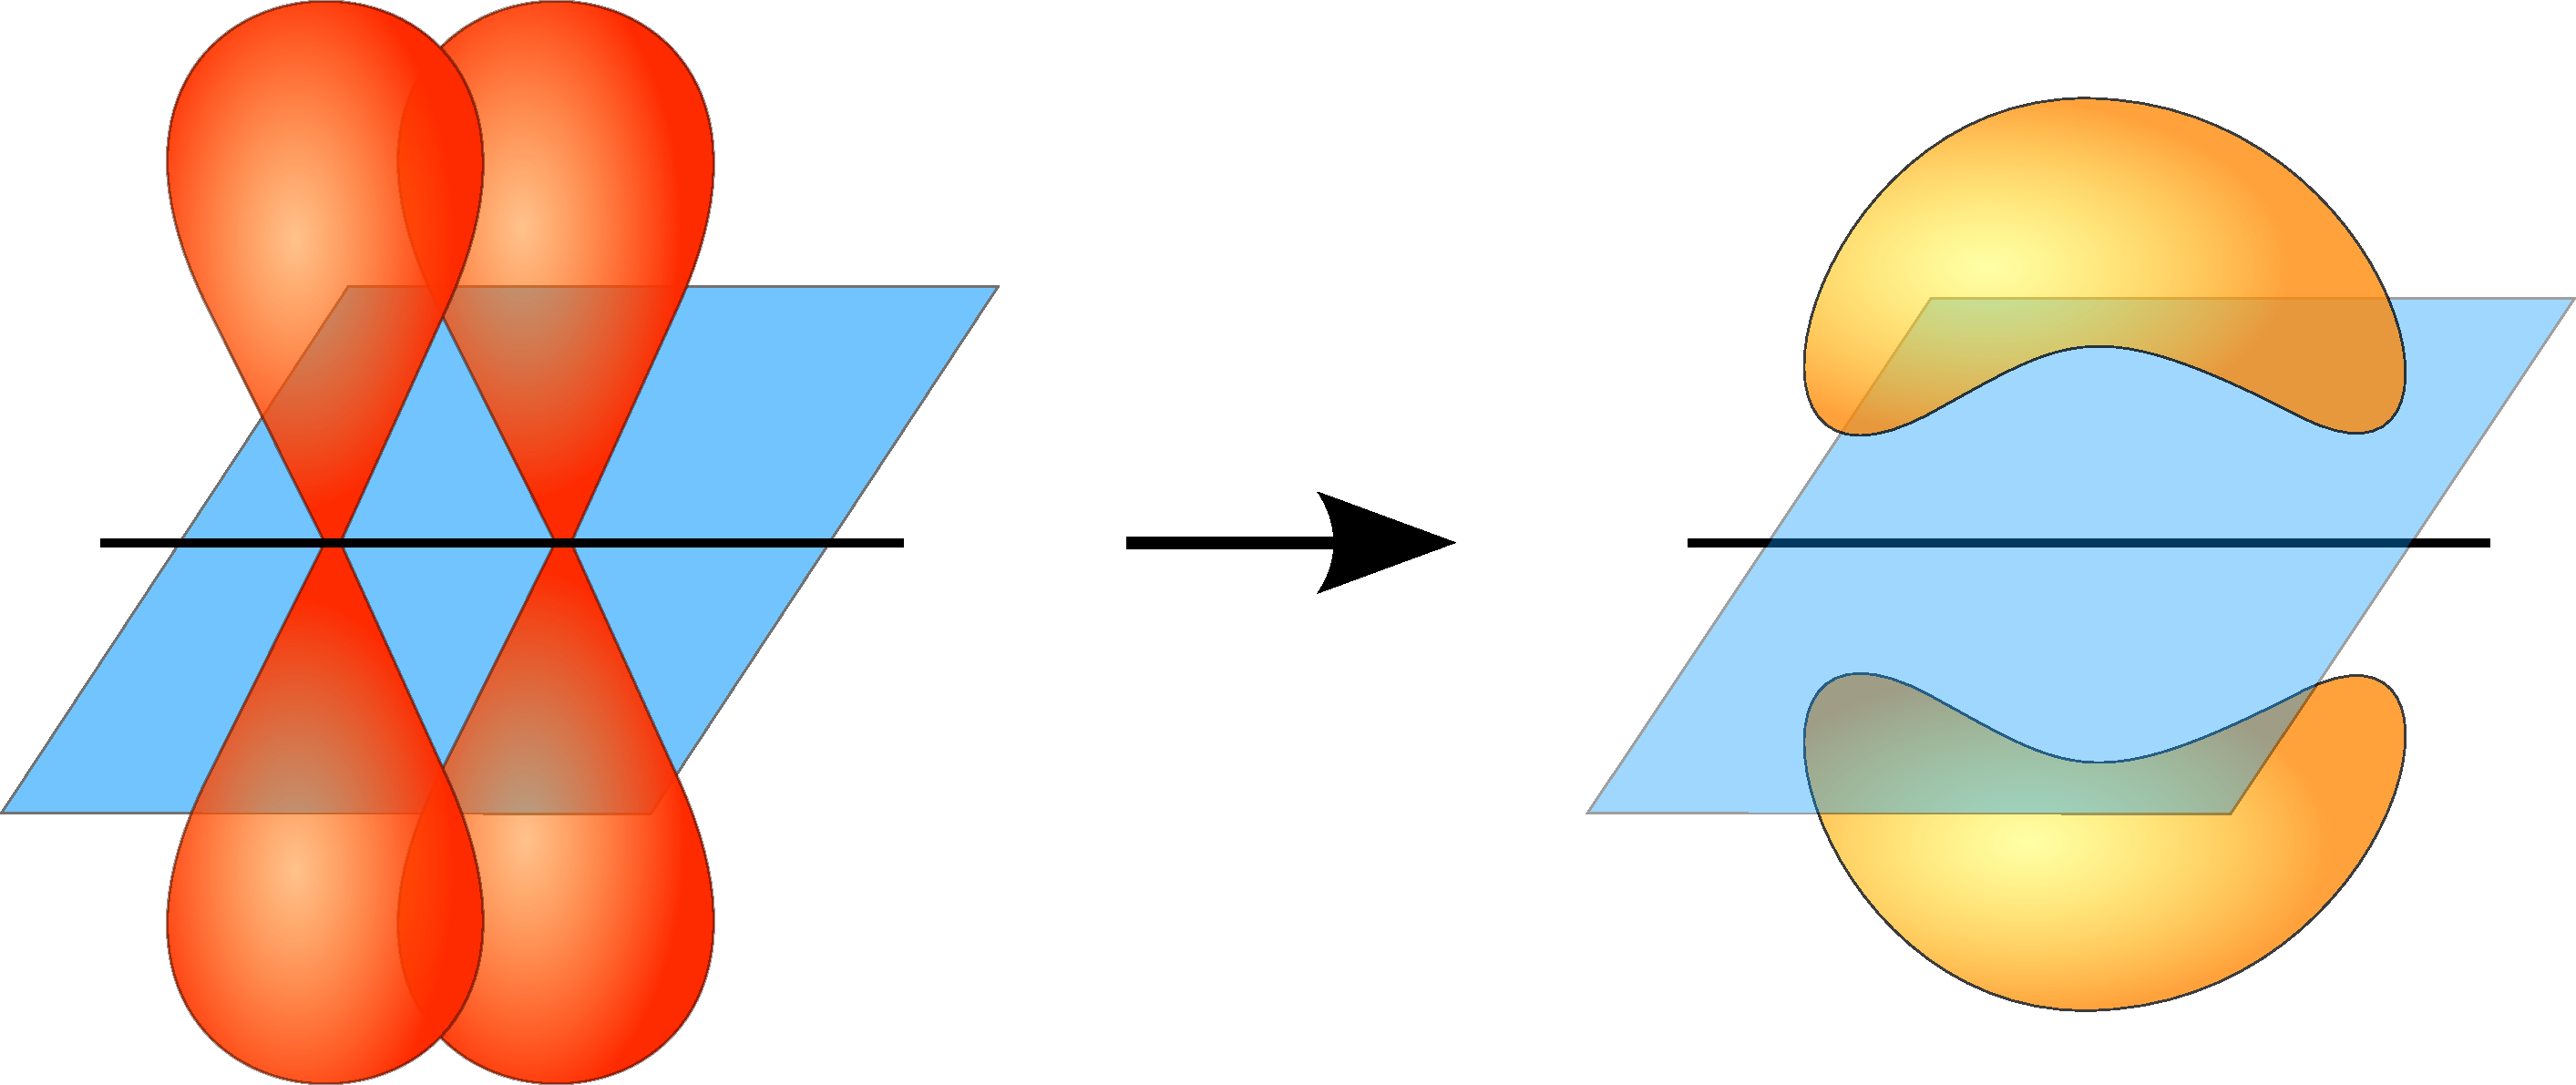
\includegraphics[scale=0.15]{images/pi-bond.pdf}
                \end{center}
                \end{itemize}
        \end{itemize}
    {\color{G-Moon}\item What is a nucleophile?}
        \begin{itemize}
            \item {\color{o-Sun}\textbf{all of the above}}
                \begin{itemize}
                    \item a nucleophile is an electron rich atom that is capable of {\color{o-Sun}donating a pair of electrons}, which is the same definition as a {\color{neg}Lewis base}.
                    \item Electron {\color{o-Sun}rich} means {\color{neg}Lewis bases are negative} and thus attracted to a {\color{pos}positive charged} center (nuclei are generally positively charged) and capable of forming a bond due to excess of electrons. 
                \end{itemize}
        \end{itemize}
    {\color{G-Moon}\item What is an electrophile?}
        \begin{itemize}
        {\color{G-Moon}\item[a.] a species that is attracted to a negative charge
            \item[b.] a species that contains extra electrons 
            \item[c.] a Lewis acid}
            {\color{o-Sun}\item[d.] \textbf{a and c}}
            \begin{itemize}
                \item An electrophile is an {\color{o-Sun}electron-deficient} atom that is capable of {\color{o-Sun}accepting a pair of electrons}, which is the same as a {\color{pos}Lewis acid}.
            \end{itemize}
        \end{itemize}
    \newpage
    {\color{G-Moon}\item When drawing curved arrows, the arrow head always points towards the Lewis acid.}
        \begin{itemize}
            \item {\color{o-Sun}\textbf{True}}
            \begin{itemize}
                \item \textbf{Tails} must be placed on either a bond or a lone pair.
                    \begin{itemize}
                        \item Shows the {\color{o-Sun}source}, i.e., the electron donor (base).
                        \item Electrons can only be found in lone pairs or bonds, so {\color{o-Sun}never place the tail} of a curved arrow on a {\color{pos}positive charge}.
                    \end{itemize}
                \item \textbf{Heads} must be placed so that it shows either the formation of a bond or the formation of a lone pair.
                    \begin{itemize}
                        \item Shows the {\color{o-Sun}destination}, i.e., the electron acceptor (acid).
                        \item Avoid drawing an arrow that violates the octet rule, so never draw an arrow that gives more than four orbitals to a second-row element.
                    \end{itemize}
                \end{itemize}
        \end{itemize}
    {\color{G-Moon}\item What factors contribute to making something a good EWG?}
        \begin{itemize}
            \item {\color{o-Sun}\textbf{all of the above}}
                \begin{itemize}
                    \item Both inductive and resonance effects can have an impact on electronegativity, which governs substituent effects, such as the electron withdrawing group.
                \end{itemize}
        \end{itemize}
    {\color{G-Moon}\item Given either the presence of a highly electronegative element that results in good inductive effects, or a group that, through resonance can delocalize positive charge, which has the greater effect as an EWG?}
        \begin{itemize}
            \item {\color{o-Sun}\textbf{a group that is capable of delocalizing positive charge through resonance}}
                \begin{itemize}
                    \item The spreading of $\pi$ bonds is called \textbf{delocalization}, {\color{o-Sun}which is a major stabilizing factor} since the electrons are shared between multipile atoms.
                    \item Inductive effect is due to electrons being shifted towards the more electronegative atom, but staying in the same place, provding less stability compared to resonance electron sharing.
                \end{itemize}
        \end{itemize}
    \newpage
    {\color{G-Moon}\item On your own, you can show how electron distribution in the structure below results in the delocalization of positive charge, which increases the electronegativity at the terminal carbon atom.
    \begin{center}
        \chemfig{=_[:-30]-[:30]=_[:-30]-[:30]N{\color{pos}^\oplus}(-[:90]O)=[:-30]O}
    \end{center}}
    \begin{itemize}
        \item I briefly read some sections on resonance, not expecting it to be on this quiz much since he talked about it very little. I'm not super confident in my explanation but I'll give it shot.
        \item There are some patterns for identifying lone pairs of oxygen and nitrogen, excerpt from todays notes:
            \begin{itemize}
                \item \textbf{Associated Patterns for Oxygen}
                \begin{itemize}
                    \item A {\color{neg}negative ($\circleddash$)} charge corresponds with {\color{o-Sun}one bond} and {\color{o-Sun}three lone pairs}.
                    \item The {\color{G-Moon}absence} of charge corresponds with {\color{o-Sun}two bonds} and {\color{o-Sun}two lone pairs}.
                    \item A {\color{pos}positive ($\oplus$)} charge corresponds with {\color{o-Sun}three bonds} and {\color{o-Sun}one lone pair} 
                \end{itemize}
            \item \textbf{Associated Patterns for Nitrogen}
                \begin{itemize}
                    \item A {\color{neg}negative} charge corresponds with {\color{o-Sun}two bond} and {\color{o-Sun}two lone pairs}.
                    \item The {\color{G-Moon}absence} of charge corresponds with {\color{o-Sun}three bonds} and {\color{o-Sun}one lone pair}.
                    \item A {\color{pos}positive} charge corresponds with {\color{o-Sun}four bonds} and {\color{o-Sun}no lone pairs}
                \end{itemize}
            \end{itemize}
        \item Thus, the nitrogen should be have a {\color{pos}positive formal} charge, due to the four bonds (including the $\pi$  bond) and no lone pairs.
        \item I don't know how to draw resonance arrows yet in the bond-line diagrams... but that charge is {\color{o-Sun}delocalized} down the carbon chain, in reality it's being shared with {\color{y-Sun}\textit{the four carbons and thus the electronegativity at the terminal carbon.\(^{?}\)}} (? Less confident about the validity of this statement, but seems reasonable)
    \end{itemize}
\end{enumerate}
\newpage
\fancyhead[L]{\hyperlink{home}{Monday, October 12}}
\subsection{Monday, October 12}
\begin{enumerate}
    {\color{G-Moon}\item How many isomers exist for a molecule with the molecular formula \ch{C4H10O}?}
        \begin{itemize}
            \item {\color{o-Sun}\textbf{7}}
                \begin{itemize}
                    \item {\tiny\chemfig{-[:30]-[:-30]-[:30]-[:-30]OH}
                          \hspace{12pt}
                          \chemfig{-[:30](-[:90])-[:-30]-[:30]OH}
                          \hspace{12pt}
                          \chemfig{-[:30]-[:-30](-[:-90])-[:30]OH}
                          \hspace{12pt}
                          \chemfig{-[:30](-[:-90])(-[:120])-[:0]OH}}
                        \begin{itemize}
                            \item These are the alcohols, or {\color{y-Sun}\textit{all the possbile combinations where the oxygen is on the end}\(^{?}\)} ({\color{y-Sun}?} I'm sure when we get into nomenclature this will make more senses and lead to better explanation)
                        \end{itemize}
                    \item {\tiny\chemfig{-[:30]-[:-30]-[:30]O-[:-30]}
                          \hspace{12pt} 
                          \chemfig{-[:30](-[:90])-[:-30]O-[:30]}
                          \hspace{12pt} 
                          \chemfig{-[:30]-[:-30]O-[:30]-[:-30]}}
                        \begin{itemize}
                            \item These are the ethers, or {\color{y-Sun}\textit{all the possbile combinations where the oxygen is within the chain}\(^{?}\)} ({\color{y-Sun}?} same disclaimer as above)
                        \end{itemize}
                    \item Seems like drawing is only way to get good at this. Eventually we will probably get some intuition or memorize certain compounds with continual practice, similar to practicing math problems.
                \end{itemize}
        \end{itemize}
    {\color{G-Moon}\item How many degrees of unsaturation are there in \ch{C4H10O}?}
        \begin{itemize}
            \item {\color{o-Sun}\textbf{0}}
                \begin{itemize}
                    \item Determining saturation using molecular formula: {\color{o-Sun}C\(_{n}\)H\(_{2n+2}\)}\\\(n=\) carbon atoms.
                        \begin{itemize}
                            \item \textbf{Halogens}: takes the place of a hydrogen atom; {\color{o-Sun}add one H} for each halogen.
                            \item \textbf{Oxygen}: no affect on saturation; {\color{o-Sun}ignore}.
                            \item \textbf{Nitrogen}: needs an extra hydrogen; {\color{o-Sun}subtract one H} for each nitrogen. 
                        \end{itemize}
                    \item Or use HDI formula: {\color{o-Sun}HDI = \(\frac{1}{2}(2C + 2 + N - H - X)~~\)} \(X\): halogen atoms.
                        \begin{itemize}
                            \item HDI: hydrogen deficiency index, which is the measure of degrees of freedom.
                            \item For \ch{C4H10O}:  \(\frac{1}{2}(8 + 2 + 0 - 10 - 0) = \frac{1}{2}(0) = 0\) 
                        \end{itemize}
                \end{itemize}
        \end{itemize}
    \newpage
    {\color{G-Moon}\item Based upon the previous question, which structure(s) can be eliminated as possible for \ch{C4H10O}?}
        \begin{itemize}
            \item {\color{o-Sun}\textbf{all of the above}}
                \begin{itemize}
                    \item {\color{o-Sun}Zero degrees of freedom} means {\color{false}no double/triple bonds or rings} are possbile.
                    \item Degrees of freedom help represent possbile structures, indicating possible double bounds, triple bounds, rings, or various combinations of each.
                \end{itemize}
        \end{itemize}
    {\color{G-Moon}\item How many degrees of unsaturation are there in \ch{C5H13}?}
        \begin{itemize}
            \item {\color{o-Sun}\textbf{0}}
                \begin{itemize}
                    \item Again, general formula: {\color{o-Sun}HDI = \(\frac{1}{2}(2C + 2 + N - H - X)~~\)} \(X\): halogen atoms.
                    \item For \ch{C5H13}{\color{true}N}:  \(\frac{1}{2}(2(5) + 2~ {\color{true}+~1} - 13 - 0) = \frac{1}{2}(0) = 0\)
                \end{itemize}
        \end{itemize}
    {\color{G-Moon}\item Based upon the previous question, what is a possible structure for \ch{C5H13N}?}
        \begin{itemize}
            \item {\color{o-Sun}\chemfig{-[:30]-[:-30]-[:30](-[:90]NH_2)-[:-30]}}
                \begin{itemize}
                    \item Same as question three, {\color{o-Sun}zero degrees of freedom} means {\color{false}no double/triple bonds or rings} are possbile.
                \end{itemize}
        \end{itemize}
    {\color{G-Moon}\item How many degrees of unsaturation exist for a molecule with the formula \ch{C3H6O2}?}
        \begin{itemize}
            \item {\color{o-Sun}\textbf{1}}
                \begin{itemize}
                    \item \(\frac{1}{2}(2(3) + 2 + 0 - 6 - 0) = \frac{1}{2}(2) = 1\)
                \end{itemize}
        \end{itemize}
    {\color{G-Moon}\item What structures are possible for the \ch{C3H6O2} molecule?}
        \begin{itemize}
            \item {\color{o-Sun}\textbf{both the first and second structures are possible}}
                \begin{itemize}
                    \item For reference: 
                    \hspace{8pt}
                    {\tiny\chemfig{-[:-30]-[:30](=[:90]O)-[:-30]OH}
                    \hspace{12pt}
                    \chemfig{-[:30](=[:90]O)-[:-30]O-[:30]}}
                    \item Has one degree of freedom so it has to have at least a double/triple bound or ring structure.
                        \begin{itemize}
                            \item Makes ~~{\tiny\chemfig{HO-[:30]-[:-30]-[:30]-[:-30]OH}} ~~invalid due to lack of any double/triple/rings.
                        \end{itemize}
                \end{itemize}
        \end{itemize}
\end{enumerate}
%\endgroup
%%%%%%%%%%%%%%%%%%%%%%%%%%%%% Week 3 %%%%%%%%%%%%%%%%%%%%%%%%%%%%%

%%%%%%%%%%%%%%%%%%%%%%%%%%%%% Week 2 %%%%%%%%%%%%%%%%%%%%%%%%%%%%%
%\begingroup
\clearpage
\section*{Week 2}\phantomsection
\addcontentsline{toc}{section}{\textbf{Week 2}}
\fancyhead[R]{\hyperlink{home}{Week 2}}


\subsection{Friday, October 9}
\fancyhead[L]{\hyperlink{home}{Wednesday, October 9}}
\begin{enumerate}
    {\color{G-Moon}\item What is the condensed formula for the following molecule?
    \begin{align*}
        \chemfig{
            {\color{b-Ocean}C}H(-[5]{\color{r-Sun}CH_3})(-[2]{\color{r-Sun}CH_3})
            (-[::-20]{\color{b-Ocean}C}H_2
            (-[::40]{\color{b-Ocean}C}(-[2]{\color{r-Sun}CH_3})(-[::-40]{\color{p-Haze}Br})(-[6]{\color{r-Sun}CH_3})
            ))
        }
    \end{align*}}
    \begin{itemize}
        \item {\color{o-Sun}\textbf{\ch{(CH3)2CHCH2C(CH3)2Br}}}
            \begin{itemize}
                \item Breaking down answer: \({\color{r-Sun}(CH_3)_2}{\color{b-Ocean}C}H{\color{b-Ocean}C}H_2{\color{b-Ocean}C}{\color{r-Sun}(CH_3)_2}{\color{p-Haze}Br}\)
            \end{itemize}
    \end{itemize}
    {\color{G-Moon}\item What is the structural formula for \ch{(CH3)3CCH(OH)CH3}? }
        \begin{align*}
            {\color{o-Sun}\chemfig{-[:30](-[:90])(-[:-90])(-[:-30](-[:-90]OH)(-[:30]))}}
        \end{align*}
        \begin{itemize}
            \item Each line with an end is a \ch{CH3} (need 4)
            \item Three points touching is a \ch{CH}. (need 1)
            \item \ch{(OH)} is on the CH
        \end{itemize}
    {\color{G-Moon}\item For any two molecules to be constitutional isomers of each other, at the very least, they:}
        \begin{itemize}
            \item {\color{o-Sun}\textbf{must have the same chemical formula}}
                \begin{itemize}
                    \item isomers: same chemical formula.
                    \item constitution: ways it connects; connect must be {\color{o-Sun}different} to be a constitutional isomer.
                \end{itemize}
        \end{itemize}
    {\color{G-Moon}\item How many constitutional isomers can be formed with the molecular formula \ch{C4H10O}?}
        \begin{itemize}
            \item {\color{o-Sun}\textbf{7}}
                \begin{itemize}
                    \item See Monday, October 12 quiz. Same question asked and a better explanation given there.
                \end{itemize}
        \end{itemize}
    \newpage
    {\color{G-Moon}\item The SO2 molecule has two resonance forms, each of which is a constitutional isomer of the other. Which of the two structures shown below is the most stable?  (The S$\rightarrow$O bond is a dative bond in which both bonding electrons come from only one atom.) }
        \begin{itemize}
            \item {\color{o-Sun}\textbf{the structure on the right}}
                \begin{itemize}
                    \item {\color{y-Sun}\textit{Delocalized electrons being shared in multiple bonds are more stable than a the dative bond.}\(^{?}\)} (? Not sufficient enough information yet to be confident of this explanation, though I'd be willing to bet that its along the right lines)
                \end{itemize}
        \end{itemize}
\end{enumerate}

\newpage
\subsection{Wednesday, October 7}
\fancyhead[L]{\hyperlink{home}{Wednesday, October 7}}
\begin{enumerate}
    {\color{G-Moon}\item What is the hybridization of the orbitals on C in ethylene?}
        \begin{itemize}
            \item {\color{o-Sun}\textbf{sp\(\bm{^{2}}\)}}
            \begin{itemize}
                \item $\chemfig{C(-[5]H)(-[3]H)(=[0]C(-[-1]H)(-[9]H))}$
                \item Each C has 3 groups (number of bonds, $\pi$ bonds count as 1, or lone pairs)
                \item For atoms with groups between 1 and 4; sp{\color{o-Sun}\(^{x}\)}; x = groups - 1 = ({\color{o-Sun}2})
            \end{itemize}
        \end{itemize}
    {\color{G-Moon}\item What is the hybridization of the orbitals on C in acetylene?}
        \begin{itemize}
            \item {\color{o-Sun}\textbf{sp}}
                \begin{itemize}
                    \item $\chemfig{C(-[4]H)(~[0]C(-[0]H))}$
                    \item 2 groups, thus x = 1.
                \end{itemize}
        \end{itemize}
    {\color{G-Moon}\item What type of bonds combine to make a C=C double bond?}
        \begin{itemize}
            \item {\color{o-Sun}\textbf{one sigma and one pi bond.}}
                \begin{itemize}
                    \item First bond is a $\sigma$ bond.
                    \item Additional bonds are $\pi$ bonds that go above and below the axis that connects the nuclei.
                \end{itemize}
        \end{itemize}
    {\color{G-Moon}\item What is the H-C-H bond angle in ethylene?}
        \begin{itemize}
            \item {\color{o-Sun}\textbf{120}$^{\bm{\,\circ}}$}
                \begin{itemize}
                    \item sp\(^{2}\) with no lone pairs, thus trigonal planar (according to VSEPR).
                    \item \(\frac{360}{3}\) = 120; 3 angles maximized on a single plane. 
                \end{itemize}
        \end{itemize}
    {\color{G-Moon}\item Why is the geometry around the CH2 fragment in ethylene, trigonal  planar?}
        \begin{itemize}
            \item {\color{o-Sun}\textbf{there are three regions of electron density}}
                \begin{itemize}
                    \item \textit{regions electron density =\(^{?}\) groups} (? I'm combining a past youtube video with his lecture...)
                \end{itemize}
        \end{itemize}
    {\color{G-Moon}\item There is completely free rotation around a sigma bond such as a \ch{C-C} single bond. Propose a reason for why there is no free rotation around a \ch{C=C}.}
        \begin{itemize}
            \item {\color{o-Sun}\textbf{the rotation would require the \ch{C-C} pi bond to break}}
                \begin{itemize}
                    \item $\sigma$ bonds can rotate on the axis between the nuclei, but the $\pi$ bonds are above and below and would break during rotation since \textit{there are other orbitals that would block\(^{?}\) their rotation}. (? not completely sure on the mechanism that doesn't allow for rotation)
                \end{itemize}
        \end{itemize}
    {\color{G-Moon}\item As the percent s character increases in a bond, what happens to the bond angle?}
        \begin{itemize}
            \item {\color{o-Sun}\textbf{it increases}}
                \begin{itemize}
                    \item The more {\color{o-Sun}\textit{s} character}, the {\color{pos}shorter} and {\color{pos}stronger} the bond, and the {\color{pos}larger} the bond angle.
                \end{itemize}
        \end{itemize}
    {\color{G-Moon}\item As the percent p character in a bond increases, what happens to the bond angle?}
        \begin{itemize}
            \item {\color{o-Sun}\textbf{it decreases}}
                \begin{itemize}
                    \item the more p character, the less s character; inverse of s character.
                \end{itemize}
        \end{itemize}
    {\color{G-Moon}\item Why is a pi bond weaker than a sigma bond?}
        \begin{itemize}
            \item {\color{o-Sun}\textbf{all of the above}}
        \end{itemize}
    {\color{G-Moon}\item Which statement(s) is(are) correct?}
        \begin{itemize}
            {\color{G-Moon}\item the shorter the bond, the stronger the bond
            \item the more s character in the hybridization, the stronger the bond
            \item the more s character in the hybridization, the greater the bond angle
            \item sigma bonds are stronger than pi bonds
            \item the geometry around the C in the ethylene is trigonal planar
            \item a \ch{C=C} bond is composed of one sigma and one pi bond
            \item the hybridization around C in the methyl anion, isoelectronic with \ch{CH4}, is sp\(^{3}\)
            \item when 2s and 2p orbitals mix to form hybrid orbitals, the hybrid orbitals are higher in energy than the 2s orbitals, but lower in energy than the 2p orbitals
            \item the shapres of the hybrid orbitals match the electron domain geometry shapes predicted by VSEPR
            \item the potential energy of a covalent bond is lower than that of the potential energies of the free atoms from which it was formed}
            \item {\color{o-Sun}\textbf{ALL OR THE ABOVE}}
            \begin{itemize}
                \item This seems to be a review of important concepts.
            \end{itemize}
        \end{itemize}
\end{enumerate}

\newpage
\fancyhead[L]{\hyperlink{home}{Monday, October 5}}
\subsection{Monday, October 5}
\begin{enumerate}
    {\color{G-Moon}\item The concept of orbital shapes comes directly from the wave model of the atom.  What is the shape of an s orbital?}
        \begin{itemize}
            \item {\color{o-Sun}\textbf{Spherical}}
                \begin{itemize}
                    \item S orbital is the most simple orbital, with only two electrons. 
                    \item Alternative shapes come from \textit{nodes}; i.e. when \textit{destructive interferences} cancels out the wave function.
                    \item Not circular, orbitals are three-dimensional.
                \end{itemize}
        \end{itemize}
    {\color{G-Moon}\item What is the shape of a p orbital?}
        \begin{itemize}
            \item {\color{o-Sun}\textbf{Dumbell shaped}}
                \begin{itemize}
                    \item P orbital can hold 6 electrons (3 pairs).
                    \item Each pair has one angular node, squeezing shape into dumbell in each direction (x, y, z).
                \end{itemize}
        \end{itemize}
    {\color{G-Moon}\item When atomic orbitals overlap to form a covalent bond, the resultant bonding orbital is:}
        \begin{itemize}
            \item {\color{o-Sun}\textbf{Lower in energy than the atomic orbitals from which it was formed}}
                \begin{itemize}
                    \item Electrons in a covalent bond are in a more stable (lower energy) state due to multiple nuclei hodling them in place.
                    \item Only when nodes are present do the electrons create a destabalized molecular orbit, incraseing the energy.
                \end{itemize}
        \end{itemize}
    {\color{G-Moon}\item Why can't pure p orbitals be used in forming four equivalent bonds as in methane?}
        \begin{itemize}
            {\color{G-Moon}\item the three 2p orbitals can only hold 6 electrons.}
                \begin{itemize}
                    \item True, we need to make four bonds for methane.
                \end{itemize}
                {\color{G-Moon}\item the bonds would have to be \ang{90} apart.}
                \begin{itemize}
                    \item If p had enough space then it would result in planar geometry with \ang{90}, but the true arrangement is tetrahedral with angles of \ang{109.5}
                \end{itemize}
                {\color{G-Moon}\item electron-electron repulsion would not be minimized.}
                \begin{itemize}
                    \item Planar minimization would be \ang{90}, but we have 3d space to work with, so it's not minimized.
                \end{itemize}
            \item {\color{o-Sun}\textbf{all of the above}}
        \end{itemize}
    {\color{G-Moon}\item When s and p orbitals combine to form hybrid orbitals, the resultant hybridized orbitals are:}
        \begin{itemize}
           {\color{G-Moon}\item lower in energy than the p orbitals
            \item higher in energy than the s orbitals}
            \item {\color{o-Sun}\textbf{both of the above}}
                \begin{itemize}
                    \item It takes energy to move the electron up from the \textit{s} orbital and hybridize the \textit{p} orbitals. 
                    \item The new hybridized sp orbital also has more energy than the s orbital.
                \end{itemize}
        \end{itemize}
    {\color{G-Moon}\item What is the difference between a sigma bond and a pi bond?}
        \begin{itemize}
            \item {\color{o-Sun}\textbf{in a $\pi$ bond, electron density lies above and below the axis that conects the two nuclei; in a $\sigma$ bond, the electronegative density lies along the axis that connets the two nuclei}}
                \begin{itemize}
                    \item $\sigma$ bond has circular symmetry with respect to the bond axis (axis that connets the two nuclei). i.e. it's along the axis.
                \end{itemize}
        \end{itemize}
    {\color{G-Moon}\item What is the hybridization of the C in CH2Cl2?}
        \begin{itemize}
            \item {\color{o-Sun}\textbf{sp\(\bm{^{3}}\)}}
                \begin{itemize}
                    \item $\chemfig{C(-[4]Cl)(-[0]Cl)(-[2]H)(-[6]H)}$
                    \item Look at central atom --- C
                    \item Determin groups (number of bonds, $\pi$ bonds count as 1, and lone pairs attached) --- 4 
                    \item for groups 1-4; sp{\color{o-Sun}\(^{x}\)}; x = groups - 1 ({\color{o-Sun}3})
                \end{itemize}
        \end{itemize}
    {\color{G-Moon}\item What is the hybridization of each C in benzene (shown below)?}
        \begin{itemize}
            \item {\color{o-Sun}\textbf{sp\(\bm{^{2}}\)}}
                \begin{itemize}
                    \item Each carbon has 2H and $\pi$ bond between, so groups = 3.
                    \item Groups - 1 = 2, so sp\(^{2}\)
                    \item Though, each $\pi$ bond is delocalized, or free to spread across all the carbons. Still counts as 1 group.
                \end{itemize}
        \end{itemize}
\end{enumerate}

%\endgroup
%%%%%%%%%%%%%%%%%%%%%%%%%%%%% Week 2 %%%%%%%%%%%%%%%%%%%%%%%%%%%%%

%%%%%%%%%%%%%%%%%%%%%%%%%%%%% Week 1 %%%%%%%%%%%%%%%%%%%%%%%%%%%%%
%\begingroup
\clearpage
\section*{Week 1}\phantomsection
\addcontentsline{toc}{section}{\textbf{Week 1}}
\fancyhead[R]{\hyperlink{home}{Week 1}}
\subsection{Friday, October 2}
\begin{itemize}
    \item Determing formal charge:
    \begin{itemize}
        \item Formula: {\color{o-Sun}\(FC = V - N - \dfrac{B}{2}\)}
        \item V = valance electrons of element
        \item N = lone pair electrons; B = bonded electrons
    \end{itemize}
    \item[1.] What is the formal charge on P in the following structure?  Each F and O has three lone pair of electrons.
        \begin{itemize}
            \item P = 5 - O - 8(0.5); P = {\color{pos}+1}
        \end{itemize}
    \item[2.] What is the formal charge on O in the structure above?
        \begin{itemize}
            \item O = 6 - 6 - 2(0.5); O = {\color{neg}-1}
        \end{itemize}
    \item[3.] What is the formal charge on P in the following structure?  Each F still has three lone pairs of electrons, and O had the tow pairs indicated.
        \begin{itemize}
            \item P = 5 - 0 - 10(0.5); P = \textbf{0}
        \end{itemize}
    \item[4.] Of the two structures shown for \ch{POF3}, which is the most stable, and will, therefore, be the most abundant form?
        \begin{itemize}
            \item \textbf{Structure II}
            \item \ch{O} has formal charge of \textbf{0} and is the 
            {\color{neg}most electronegative} element with difference in charge between the resonance structures.
            \item \ch{F} has greater electronegativity, but remains the same between both structures, so it's not relevant.
            \item Key difference: the double bond in structure II gives oxygen the {\color{o-Sun}lower magnitude} formal charge between the two.
        \end{itemize}
    \item[5.] The fundamental concept upon which VSEPR, and hence molecular shapes, is based is that:
        \begin{itemize}
            \item Electrons pairs repel each other;
                \begin{itemize}
                    \item negative charge repels other negative charges.
                \end{itemize}
            \item Electron repulsion is minimized by maximum angular separation; 
                \begin{itemize}
                    \item in other words, angular separation maximizes distance between electrons.
                \end{itemize}
            \item Bonding pair electrons and lone pair electrons both occupy regions around the central atom;
                \begin{itemize}
                    \item if they didn't occupy the same space than they wouldn't interact and thus wouldn't affect shape.
                \end{itemize}
            \item The electron dommain geometry and the molecular geometry is identical if there all of the electrons are bonding electrons;
                \begin{itemize}
                    \item the lone pairs are have a greater influence than bonded pairs, resulting in less space for bonded pairs.
                \end{itemize}
            \item \textbf{All of the above}
        \end{itemize}
    \item General method of determining structure:
    \begin{itemize}
        \item[1.] Count steric number---the total number of electron pairs in a molecule. Can be bonds or lone pairs.
        \item[2.] Determine predicted geomterical structure predicted (EDG) by VSEPR using steric number.
            \begin{itemize}
                \item Octahedral:6, Bipyramid:5, Tetrahedral:4, Trigonal:3, Linear:2
            \end{itemize}
        \item[3.] Determin impact (the MG) of lone pairs; more lone pairs results in less space between bonded pairs. Shape depends on EDG.
    \end{itemize}
    \item[6.] A resonance form of \ch{SOF2}, completely consistent with the octet rule,  is shown below.  What is the electron domain geometry (EDG), and molecular geometry (MG) of this molecule?
        \begin{itemize}
            \item \textbf{Tetrahedral EDG and trigonal pyramidal MG}
        \end{itemize}
    \item[7.] Draw a Lewis dot structure of formaldehyde (\ch{CH2O}): what is the molecular shape of this molecule?
        \begin{align*}
            \chemfig{C(=[2,]O)(-[5]H)(-[7]H)}
        \end{align*}
        \begin{itemize}
            \item Steric number = 3
                \begin{itemize}
                    \item Double bonds count as 1 for steric number.
                \end{itemize}
            \item No lone pairs on central atom, C, so it's shape planar. 
            \item \textbf{Trigonal planar}
        \end{itemize}
    \item[8.] The EDG for \ch{CH3-} (a carbanion) is tetrahedral, and the MG is trigonal pyramidal.  Why are the \ch{H-C-H} bond angles less than \ang{109.5} as in a perfect tetrahedron? 
        \begin{itemize}
            \item \textbf{The lone pair electrons take up more space than bonding pair electrons.}
        \end{itemize}
\end{itemize}
%\endgroup
%%%%%%%%%%%%%%%%%%%%%%%%%%%%% Week 1 %%%%%%%%%%%%%%%%%%%%%%%%%%%%%


\end{document}